\subsection{BLDC Regelung}\label{Trapezfoermige Regelung}
%%BLDC Motor wird auch Blockstrommotor genannt
	BLDC-Motoren werden meistens mit einem einfachen Regler bestehend aus 6 MOSFETs geregelt. Mithilfe von diesen kann jede Phase des Motors auf entweder VCC(Versorgungsspannung) oder GND(Nullpotenzial) geschalten werden. 
	
	\begin{figure}[H]
			\centering
			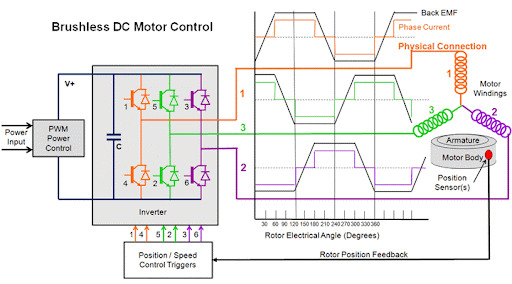
\includegraphics[scale=0.7]{./3_Stand_der_Technik/Abbildungen/BLDC_Control_3}
			\caption{BLDC-Regler\cite{settech.com.tw2024}}
	\end{figure}
	
	\begin{figure}[H]
			\centering
			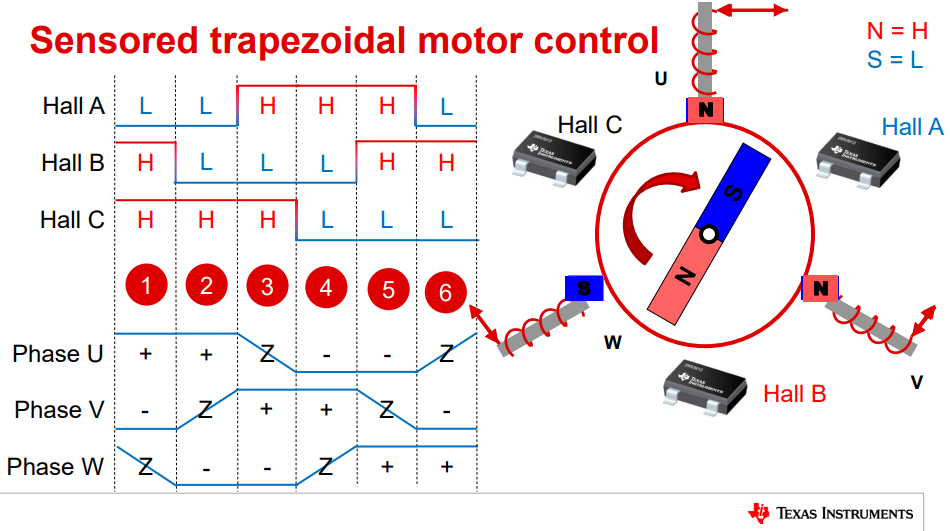
\includegraphics[scale=0.5]{./3_Stand_der_Technik/Abbildungen/BLDC_Control_4}
			\caption{Eine Rotation\cite{settech.com.tw2024}}
	\end{figure}
	
	Zus�tzlich zu den 6 MOSFETs besteht die Schaltung aus einigen Komponenten zur Spannungsstabilisierung und aus einer Kontrolleinheit. Diese Kontrolleinheit misst die Rotoposition(siehe \ref{Positionsmessung}) und schaltet die MOSFETs dementsprechend. Dadurch entsteht ein sechs-stufiger Ablauf. Die Anzahl an Positionen, die ein Motor mithilfe dieser Regelmethode annehemen kann, ergibt sich aus dem sechsfachen der Polpaare des Motors. Im Optimalfall sollte das Rotorfeld dem Statorfeld um 90� vorlaufen um maximales Drehmoment zu erzeugen. Bei dieser Regelung variiert es jedoch immmer zwischen 60� und 120�, was dazu f�hrt, dass das Drehmoment im Laufe einer Rotation merhmals zu- und abnimmt. Auch die Geschwindigkeit ist w�hrend einer Umdrehung nicht ganz konstant.
	
	\begin{figure}[H]
			\centering
			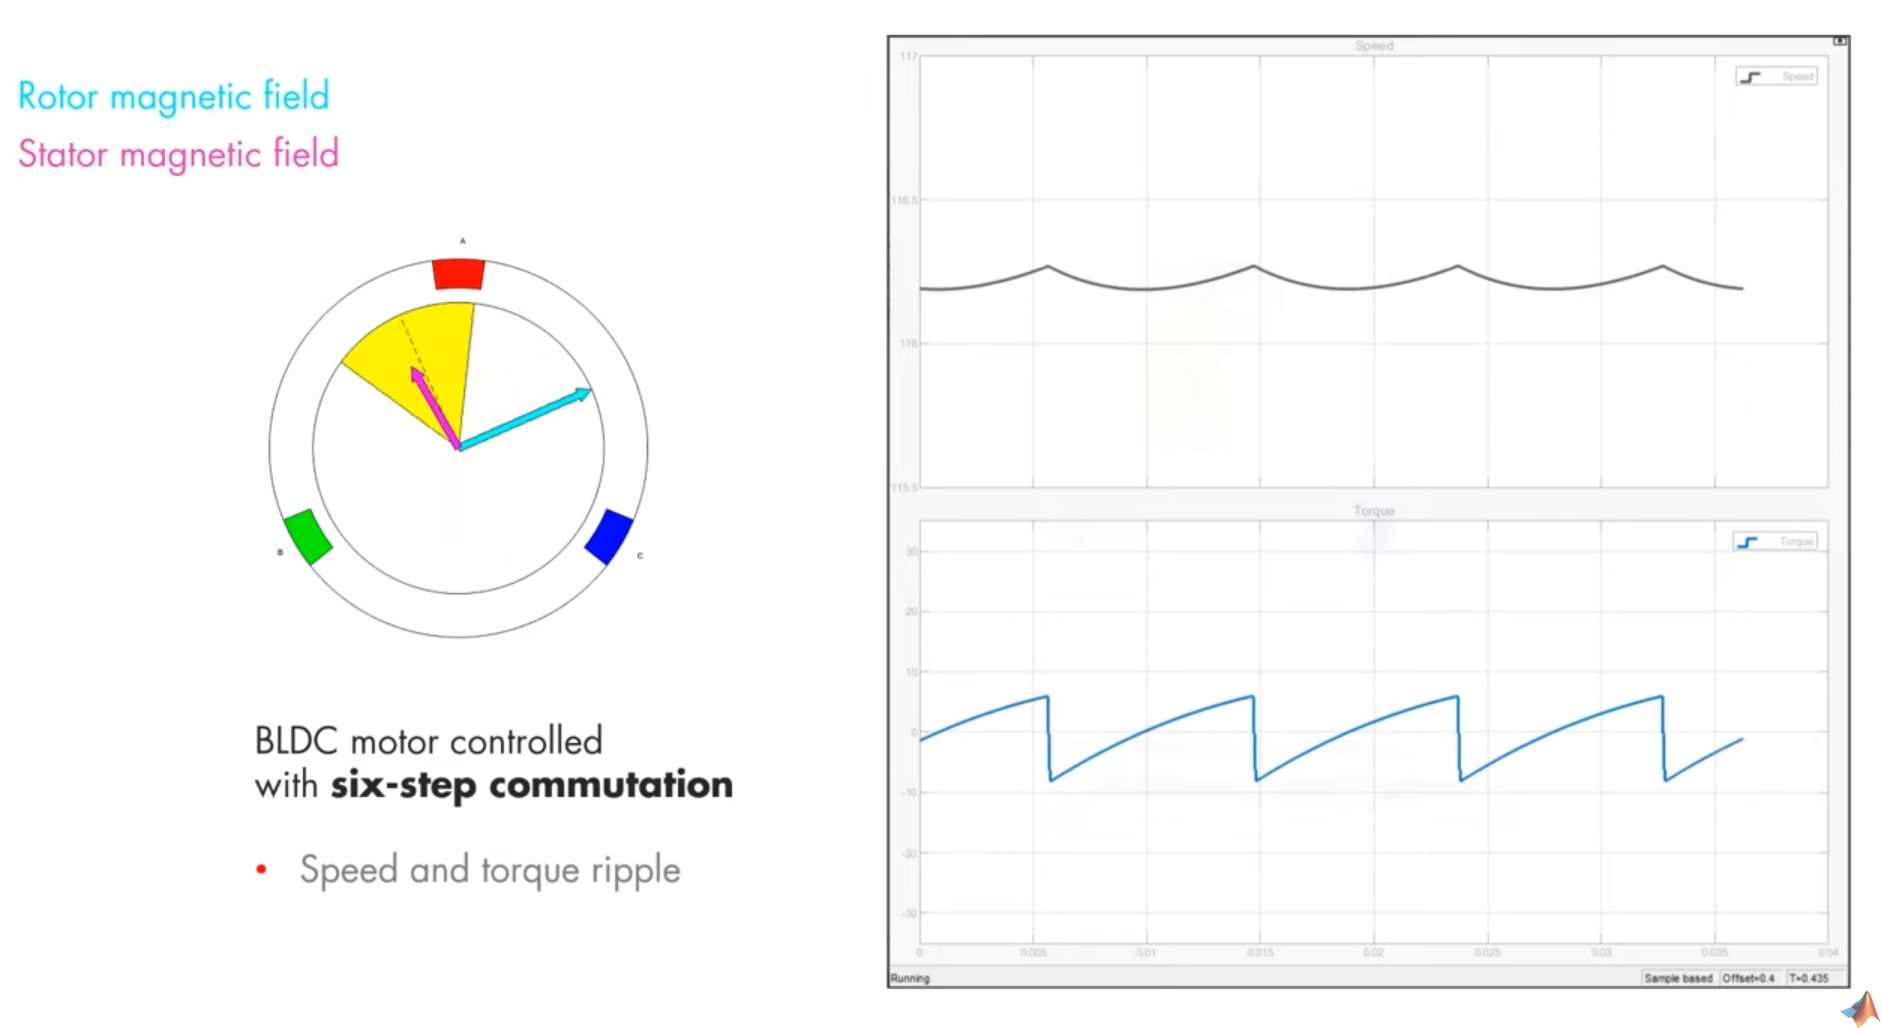
\includegraphics[scale=0.3]{./3_Stand_der_Technik/Abbildungen/BLDC_Control_1}
			\caption{Feld und Drehmoment bei BLDC-Regelung\cite{MATLAB2020}}
	\end{figure}
	
	Je nach gew�nschter Drehzahl(beziehungsweise Duty-Cycle) werden die MOSFETs, welche VCC anlegen immer l�nger eingeschaltet als die, die GND anlegen, bei 100\% Duty Cylce sind also nur die HIGH-Side(VCC) MOSFETs aktiv, bei 0\% nur die LOW-Side(GND) MOSFETs.